%Capítulo 3

\section{Diseño de la propuesta}

    La parte del backend del sistema de investigadores se compondrá de la siguiente figura \ref{fig:architecture}:
    
    \begin{figure}[H]
        \centering
        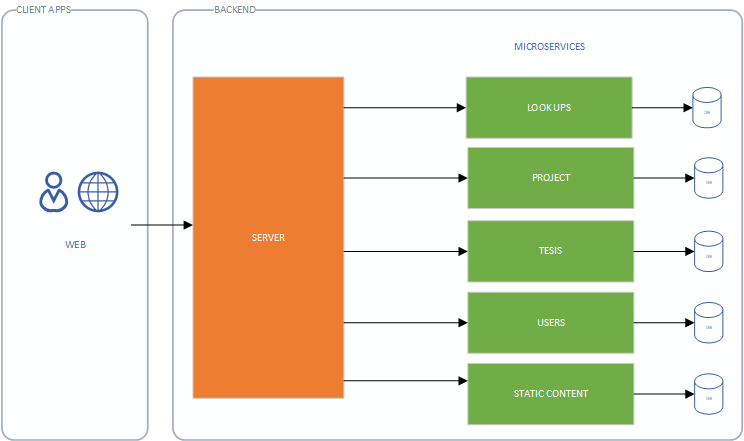
\includegraphics[width=\textwidth]{Propuesta_Plantilla_Tesis_LaTeX_UAG/imagenes/ARCHITECTURE.png}
        \caption{Arquitectura del sistema de investigadores.}
        \label{fig:architecture}
    \end{figure}
    
    Con base en la figura \ref{fig:architecture} podemos apreciar que el backend va a responder a una petición hecha a través del usuario usando una interfaz gráfica, acto seguido el servidor identificará la petición para direccionarla al micro servicio correspondiente y esta hará una consulta a la base de datos para poder satisfacer la petición.
    
    Hay distintos tipos de petición que un usuario puede realizar al backend, dentro de estos se encuentran los siguientes verbos o métodos HTTP:
    
    \begin{itemize}
        \item GET: Se utiliza como lectura de datos.
        \item POST: Para poder crear nuevas entradas en la base de datos.
        \item PUT: Para la modificación de datos.
        \item DELETE: Para el borrar datos.
    \end{itemize}
    
    Los distintos tipos de usuarios que existirán son dos: Alumno e Investigador, los cuales tendrán diferentes tipos de participaciones dependiendo del trabajo al que se asignen; mostrados en la figura \ref{fig:users_table}.
    
    \begin{figure}[H]
        \centering
        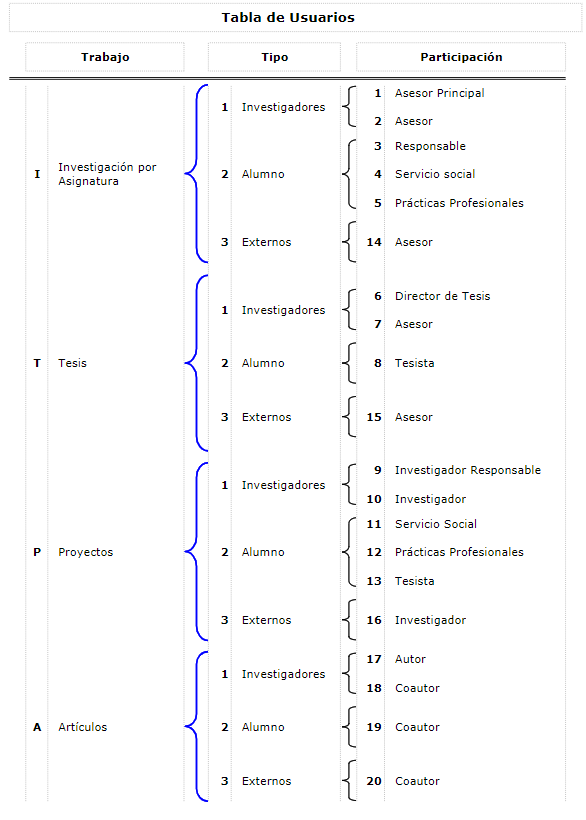
\includegraphics[width=\textwidth]{Propuesta_Plantilla_Tesis_LaTeX_UAG/imagenes/tabla_usuarios.png}
        \caption{Tabla de usuarios ordenada por trabajo y tipo de participación.}
        \label{fig:users_table}
    \end{figure}
    
    Dentro de los posibles flujos para un usuario que quiere consultar todas las tesis registradas para un alumno se puede apreciar en la figura \ref{fig:getAllTesisFromStudents} y sus pasos son los siguientes:
    
    \begin{enumerate}
        \item Realizar la petición al servidor.
        \item El servidor direccionará la petición al micro servicio o API correspondiente por medio de la URI.
        \item El micro servicio resolverá la petición del usuario y dará una respuesta con base en los datos proporcionados en la petición.
        \item El servidor obtendrá la respuesta y la regresará al usuario a través del frontend.
    \end{enumerate}
    
    \begin{figure}[H]
        \centering
        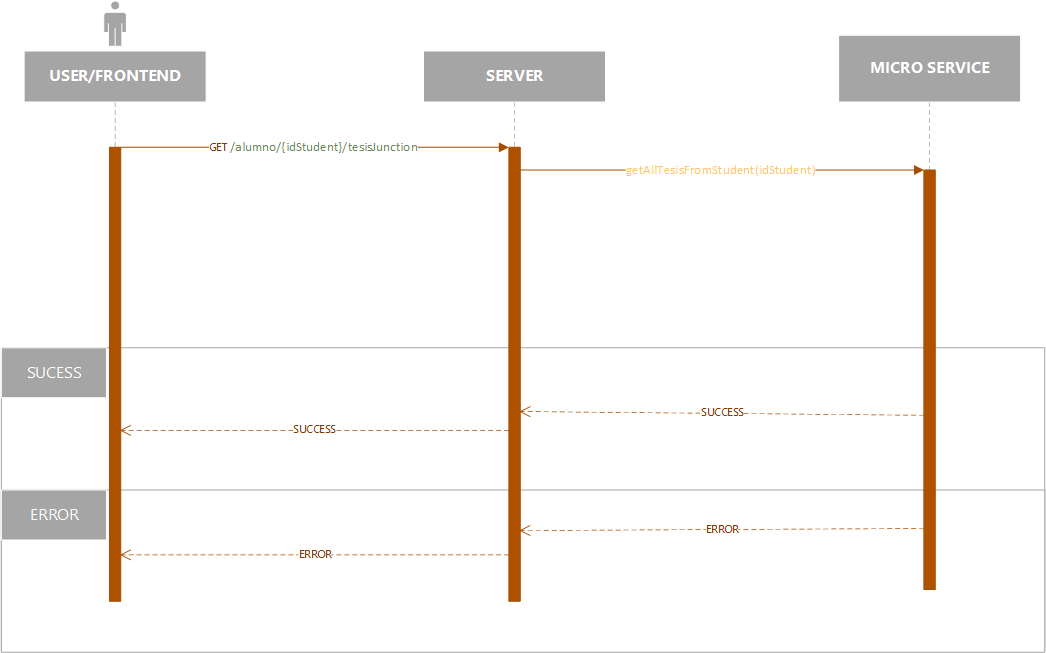
\includegraphics[width=\textwidth]{Propuesta_Plantilla_Tesis_LaTeX_UAG/imagenes/getAllTesisFromStudents_sequence_diagram.png}
        \caption{Diagrama UML para la secuencia de obtener las tesis de un alumno.}
        \label{fig:getAllTesisFromStudents}
    \end{figure}

\section{Metodología}

    La forma de trabajar se basa en metodologías ágiles, las cuales se hacen iteraciones pequeñas para presentar entregables de manera constante y obtener retroalimentación de la Doctora Lina María Aguila Lobo, la cual representa en este grupo de trabajo al cliente y sus necesidades. Las metodologías ágiles tienen un manifiesto\cite{AgileManifesto}:
    
    \begin{itemize}
        \item Individuos e interacciones sobre procesos y herramientas. \cite{AgileManifesto}
        \item Software funcionando sobre documentación extensiva. \cite{AgileManifesto}
        \item Colaboración con el cliente sobre negociación contractual. \cite{AgileManifesto}
        \item Respuesta ante el cambio sobre seguir un plan. \cite{AgileManifesto}
    \end{itemize}
    
    Además de que las metodologías ágiles se basan en 12 principios\cite{AgilePrinciples}:
    
    \begin{enumerate}
        \item Nuestra mayor prioridad es satisfacer al cliente mediante la entrega temprana y continua de software con valor. \cite{AgilePrinciples}

        \item Aceptamos que los requisitos cambien, incluso en etapas tardías del desarrollo. Los procesos Ágiles aprovechan el cambio para proporcionar ventaja competitiva al cliente. \cite{AgilePrinciples}

        \item Entregamos software funcional frecuentemente, entre dos semanas y dos meses, con preferencia al periodo de tiempo más corto posible. \cite{AgilePrinciples}

        \item Los responsables de negocio y los desarrolladores trabajamos juntos de forma cotidiana durante todo el proyecto. \cite{AgilePrinciples}

        \item Los proyectos se desarrollan en torno a individuos motivados. Hay que darles el entorno y el apoyo que necesitan, y confiarles la ejecución del trabajo. \cite{AgilePrinciples}

        \item El método más eficiente y efectivo de comunicar información al equipo de desarrollo y entre sus miembros es la conversación cara a cara. \cite{AgilePrinciples}

        \item El software funcionando es la medida principal de progreso. \cite{AgilePrinciples}

        \item Los procesos Ágiles promueven el desarrollo sostenible. Los promotores, desarrolladores y usuarios debemos ser capaces de mantener un ritmo constante de forma indefinida. \cite{AgilePrinciples}

        \item La atención continua a la excelencia técnica y al buen diseño mejora la Agilidad. \cite{AgilePrinciples}

        \item La simplicidad, o el arte de maximizar la cantidad de trabajo no realizado, es esencial. \cite{AgilePrinciples}

        \item Las mejores arquitecturas, requisitos y diseños emergen de equipos auto organizados. \cite{AgilePrinciples}
        
        \item A intervalos regulares el equipo reflexiona sobre cómo ser más efectivo para a continuación ajustar y perfeccionar su comportamiento en consecuencia. \cite{AgilePrinciples}
    \end{enumerate}
    
    Tomando en cuenta la forma de trabajar de la metodología ágil el desarrollo del sistema de investigadores se realiza de la siguiente manera: cada iteración durará una semana, por lo que se deben de presentar entregables al lunes de cada semana siguiente, en el lunes que se presentan entregables se hará una junta de 1 hora máximo para mostrar avances que se hayan dado en la semana anterior, coordinar los esfuerzos para elegir y comprometerse a terminar por cada integrante del equipo basándose en las tareas pendientes, además de que en la junta se tratan temas para apoyar a integrantes del equipo que puedan estar atorados en alguna tarea debido a que esta sea compleja o se requiera de obtener información adicional.
    
    La manera de llevar un control y seguimiento del progreso del sistema de investigadores es a través de un sistema llamado Jira, el cual permite crear tareas nuevas, asignarlas a cualquier integrante del equipo, cerrarlas para que se pueda determinar el avance real de el sistema de investigadores y, dar visibilidad al progreso total del equipo.
    
    Cada actividad o tarea realizada es evaluada o supervisada por otro integrante del equipo, lo cual ayuda a validar y verificar que lo que se está haciendo es lo pedido por la Doctora Lina María Aguilar Lobo y, que se hace de la manera correcta.
    
    Por el momento la única forma de mostrar el funcionamiento de los componentes o módulos creados es usando un ambiente local que el desarrollador tendrá instalado en su máquina.

\section{Cronograma}
Es la planificación y logística que se destinará a cada una
de las etapas de la investigación.
• Es el plan de actividades que muestra un orden lógico y
secuencial del proceso del proyecto.
• Deben señalarse las actividades que serán necesarias
desarrollar para cada etapa de la investigación.
• Comprende desde la presentación del protocolo hasta la
entrega del borrador de tesis.
• Se deben establecer las actividades en función del tiempo
disponible, recursos, materias que se están cursando y
políticas institucionales.

Se debe realizar un calendario tentativo de las actividades
indicadas en la metodología, indicando claramente las
tareas a desarrollar, por etapas, las cuales deberán tener un
estado actualizado (en curso, concluida).
• Se debe tener en cuenta el tiempo que se dedicará a cada
actividad. Aunque parece un detalle menor, este indicará la
factibilidad de realizar el proyecto en el tiempo determinado.
• Se deben indicar las actividades secuenciales o
dependientes y simultáneas.

Debe responder, entre otras, a las siguientes preguntas:
- ¿Cuándo se hará la recopilación de datos?
- ¿Cuándo se hará el diseño y el desarrollo (hardware o
software)
- ¿Cuándo se escribirá la tesis?
- ¿Cuándo se defenderá la tesis?

\section{Entregables}

    Se consideran los siguientes productos derivados del proyecto:
    
    \begin{enumerate}
        \item Documento Final
        \item Presentación de avances en seminarios y coloquios.
        \item Manuales de procedimientos.
        \item Código
    \end{enumerate}